\documentclass[10pt,twocolumn,letterpaper]{article}

\usepackage[review]{cvpr}

\usepackage{multirow}
\usepackage{booktabs}
\usepackage{amsmath}
\usepackage{amssymb}
\usepackage{xspace}
\usepackage{graphicx}
\usepackage{subcaption}
\usepackage{xcolor}
\usepackage{colortbl}

\definecolor{cvprblue}{rgb}{0.21,0.49,0.74}
\usepackage[pagebackref,breaklinks,colorlinks,allcolors=cvprblue]{hyperref}

\newcommand{\method}{CounterBench\xspace}
\newcommand{\ccs}{CCS\xspace}

\def\paperID{****}
\def\confName{CVPR}
\def\confYear{2026}

\begin{document}

\title{CounterBench: A Controllable Counterfactual Testbed Reveals\\Systematic Reasoning Failures in Vision-Language Models}

\author{Aayam Bansal\textsuperscript{1} \and Ishaan Gangwani\textsuperscript{1}\\
\textsuperscript{1}Independent Research\\
{\tt\small \{aayambansal, ishaangangwani\}@gmail.com}}

\maketitle

%----------------------------------------------------------------------
\begin{abstract}
Vision-language models (VLMs) achieve impressive accuracy on standard visual question answering benchmarks, yet it remains unclear whether they reason about scenes or merely pattern-match from surface cues. We introduce \method, a fully synthetic, controllable benchmark for evaluating \emph{counterfactual consistency} in VLMs. For each of 550 test items, we programmatically generate a paired scene: an original and an \emph{intervened} variant where exactly one semantic property is changed (an object's position, color, count, containment, or a causal link). We pose the same question to both images and measure whether the model's answer changes \emph{if and only if} the intervention is relevant---the \emph{Counterfactual Consistency Score} (\ccs). Evaluating four state-of-the-art VLMs (GPT-4o, Gemini~2.0 Flash, Qwen2.5-VL-72B, GPT-4o~mini), we find that while all models achieve 85--91\% single-image accuracy, \ccs drops to 80--90\%, with dramatic category-specific failures: \emph{all} models score $\leq$66\% on causal arrow-following tasks, GPT-4o~mini achieves only 48\% \ccs on counting, and even the strongest model (Qwen2.5-VL) reaches only 89.5\% overall \ccs. Crucially, spatial and containment reasoning are near-perfect (97--100\%), revealing that failures are \emph{selective}, not uniform. Our results demonstrate that a cheap, fully controllable testbed---generated in minutes with standard Python libraries---can surface systematic VLM failures invisible to standard benchmarks. We release the full benchmark, generation code, and evaluation pipeline.
\end{abstract}

%----------------------------------------------------------------------
\section{Introduction}
\label{sec:intro}

The rapid progress of vision-language models (VLMs) such as GPT-4o~\cite{achiam2023gpt4}, Gemini~\cite{team2024gemini}, and Qwen2.5-VL~\cite{bai2025qwen25vl} has yielded systems that can describe complex images, answer nuanced questions, and reason about visual scenes. Yet a growing body of evidence suggests that strong benchmark performance may mask fundamental reasoning deficiencies. Winoground~\cite{thrush2022winoground} revealed near-chance compositional reasoning; the ARO benchmark~\cite{yuksekgonul2023aro} showed VLMs behave as ``bags of words''; BLINK~\cite{fu2024blink} demonstrated that even GPT-4V performs only slightly above chance on core perceptual tasks; and MMVP~\cite{tong2024mmvp} exposed ``CLIP-blind'' patterns that propagate through entire model families.

A key limitation of existing benchmarks is that they test whether models give \emph{correct answers}, but not whether models \emph{reason correctly}. A model might answer ``the ball is left of the cup'' correctly by exploiting statistical regularities in its training data, without genuinely parsing the spatial relationship. To distinguish true reasoning from pattern matching, we need \emph{counterfactual} evaluation: if we intervene on the scene---say, swap the positions of ball and cup---does the model's answer flip accordingly? And equally important: if we make an \emph{irrelevant} change (e.g., alter the background color), does the answer \emph{stay the same}?

This counterfactual framing, grounded in Pearl's interventionist theory of causation~\cite{pearl2009causality} and developmental studies of causal cognition~\cite{gopnik2004causal, spelke2007core}, provides a principled test of whether models maintain internally consistent world models. Counterfactual consistency has been studied in NLP~\cite{niu2021cfvqa} and for text-image matching~\cite{wang2023eqben, zhang2024countercurate}, but no existing benchmark provides a fully controllable, programmatically generated testbed with paired visual interventions and a formal consistency metric.

We introduce \method, a benchmark with the following properties:

\begin{enumerate}
\setlength\itemsep{0pt}
\item \textbf{Paired counterfactual design.} Each item consists of an original image and an intervened image where exactly one semantic property is changed, plus a question whose correct answer is deterministic for both images.
\item \textbf{Five cognitive dimensions.} We test spatial relations, attribute binding, counting, containment, and causal reasoning (arrow-following, occlusion, compositionality).
\item \textbf{Negative controls.} 50 items where the intervention is \emph{irrelevant} (adding a distant distractor), testing whether models maintain stability.
\item \textbf{Counterfactual Consistency Score (\ccs).} The percentage of pairs where the model answers \emph{both} the original and intervened image correctly---capturing not just accuracy but \emph{reasoning consistency}.
\item \textbf{Zero cost, full control.} All 1,100 images are generated in $<$1 minute using PIL (Python Imaging Library), with deterministic ground truth.
\end{enumerate}

Our evaluation of four VLMs reveals selective, systematic failures:
\begin{itemize}
\setlength\itemsep{0pt}
\item All models achieve near-perfect \ccs on spatial (100\%) and containment (97--100\%) tasks---these are ``solved.''
\item Causal reasoning (arrow-following) is universally weak: every model scores $\leq$66\% \ccs.
\item Counting consistency varies dramatically: Qwen2.5-VL achieves 97\% but GPT-4o~mini only 48\%.
\item Attribute binding shows unexpected model-specific failures: Gemini~2.0 Flash drops to 79\% despite strong overall accuracy.
\item The \emph{consistency gap}---the difference between single-image accuracy and \ccs---ranges from 0 to 14 percentage points, revealing that some models give correct answers to individual images but inconsistent answers across the pair.
\end{itemize}

These findings demonstrate that a cheap, fully controllable testbed---requiring no training data, no crowdsourcing, and no GPU compute---can reveal systematic VLM failures that are invisible to standard benchmarks.

%----------------------------------------------------------------------
\section{Related Work}
\label{sec:related}

\paragraph{Compositional reasoning benchmarks.}
A rich line of work probes VLM compositionality. Winoground~\cite{thrush2022winoground} uses 400 human-curated image-caption pairs requiring word-order sensitivity, finding VLMs near chance. CREPE~\cite{ma2023crepe} tests systematicity and productivity of compositionality across 370K+ pairs. SugarCrepe~\cite{hsieh2023sugarcrepe} showed that prior benchmarks were ``hackable''---text-only models could outperform VLMs---and proposed adversarial refinement. The ARO benchmark~\cite{yuksekgonul2023aro} demonstrated bag-of-words behavior with 50K+ test cases. ConMe~\cite{huang2024conme} uses VLM-to-VLM adversarial conversations to generate harder compositional challenges. These benchmarks use \emph{natural} images with text-based perturbations; by contrast, \method uses \emph{fully synthetic} images with \emph{visual} interventions, providing complete control over the counterfactual manipulation.

\paragraph{Controlled and synthetic evaluation.}
CLEVR~\cite{johnson2017clevr} pioneered programmatic scene generation for visual reasoning, though it predates modern VLMs. VisMin~\cite{awal2024vismin} generates minimal-change image pairs using diffusion models. CounterCurate~\cite{zhang2024countercurate} uses GLIGEN and DALL-E 3 for counterfactual image generation. VSR~\cite{liu2023vsr} tests spatial reasoning with natural images. Our work differs from diffusion-based approaches in that our scenes are \emph{deterministically generated} with exact ground truth---no generation artifacts, no ambiguity, and trivial to reproduce.

\paragraph{Counterfactual reasoning.}
Counterfactual VQA~\cite{niu2021cfvqa} applies causal interventions to reduce language bias in VQA. EqBen~\cite{wang2023eqben} tests equivariant similarity---whether VLM similarity scores change faithfully under semantic modifications. NaturalBench~\cite{li2024naturalbench} pairs questions with two images yielding different answers. Our \ccs metric most closely relates to EqBen's equivariance concept, but extends it from similarity scoring to open-ended question answering across multiple cognitive dimensions.

\paragraph{Cognitive evaluation of VLMs.}
BLINK~\cite{fu2024blink} reformulates classic CV tasks as VQA, finding GPT-4V at 51\% vs.\ human 96\%. MMMU~\cite{yue2024mmmu} tests expert-level reasoning across 30 subjects. POPE~\cite{li2023pope} measures object hallucination. Gavrikov~\etal~\cite{gavrikov2025talk} study texture-shape bias inheritance in VLMs. Our work contributes a cognitively-grounded evaluation that probes \emph{counterfactual} reasoning---a core capacity identified in developmental psychology~\cite{gopnik2004causal}---using a formally precise, zero-cost methodology.

%----------------------------------------------------------------------
\section{The CounterBench Benchmark}
\label{sec:method}

\subsection{Design Principles}

\method is built on four principles: (1)~\textbf{counterfactual pairing}: every test item is a paired $(I_\text{orig}, I_\text{int})$ with a shared question $q$; (2)~\textbf{deterministic ground truth}: correct answers are computed from the generation parameters, eliminating annotation noise; (3)~\textbf{minimal intervention}: each intervention changes exactly one semantic property; (4)~\textbf{full reproducibility}: the entire benchmark is generated by a single Python script with a fixed random seed.

\subsection{Scene Generation}

All scenes are 512$\times$512 pixel images with a light gray background, containing colored geometric shapes (circles, squares, triangles, diamonds) in 8 distinct colors. We use PIL (Python Imaging Library) to render shapes, containers (rectangles), arrows, and text labels. The generation script produces 1,100 images (550 original-intervened pairs) in under 60 seconds on a single CPU.

\begin{figure*}[t]
\centering
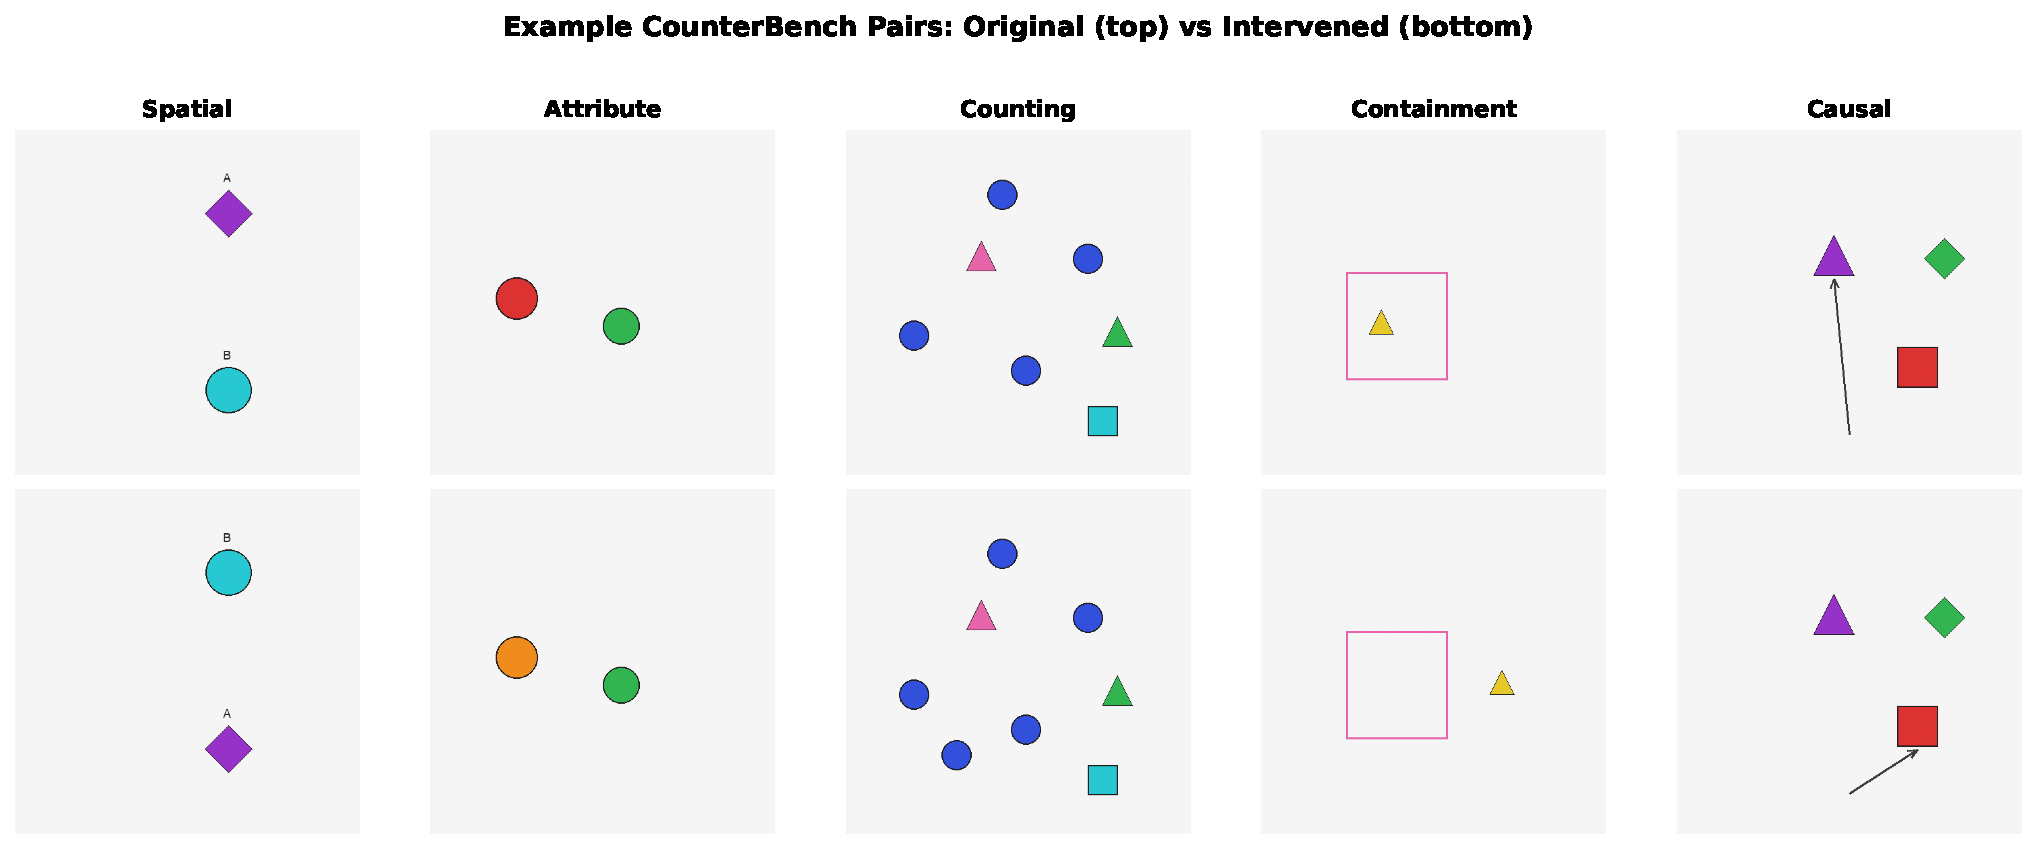
\includegraphics[width=0.95\textwidth]{../figures/example_pairs.pdf}
\caption{\textbf{Example \method pairs} across five task categories. \textbf{Top}: original scenes. \textbf{Bottom}: intervened scenes with exactly one semantic property changed. Questions and ground-truth answers are deterministic for each image.}
\label{fig:examples}
\end{figure*}

\subsection{Task Categories}

We define five task categories (100 pairs each) plus 50 negative control pairs:

\paragraph{Spatial Relations (100 pairs).} Two labeled shapes (A and B) are placed in a spatial arrangement. Question: ``Is A to the \{left/right/above/below\} of B?'' Intervention: swap the positions of A and B. Expected: answer flips from ``yes'' to ``no.''

\paragraph{Attribute Binding (100 pairs).} Multiple shapes of different colors are arranged on the canvas. Question: ``What color is the \{position\} \{shape\}?'' Intervention: change the target shape's color. Expected: answer changes to the new color.

\paragraph{Counting (100 pairs).} A target set of identical shapes and a distractor set. Question: ``How many \{color\} \{shape\}s are there?'' Intervention: add or remove one target shape. Expected: count changes by $\pm$1.

\paragraph{Containment (100 pairs).} A shape and a rectangular container. Question: ``Is the \{shape\} inside the container?'' Intervention: move the shape inside $\leftrightarrow$ outside. Expected: answer flips.

\paragraph{Causal/Compositional (100 pairs).} Three sub-tasks: (a)~\emph{Arrow pointing} (34 pairs): an arrow points to one of three shapes; intervention redirects the arrow; question asks which shape is pointed to. (b)~\emph{Occlusion} (33 pairs): two overlapping shapes; intervention removes the front shape; question asks how many shapes are visible. (c)~\emph{Compositional} (33 pairs): two shapes in a vertical arrangement; intervention swaps vertical positions; question asks about the spatial composition.

\paragraph{Negative Controls (50 pairs).} A single shape in the center. Question: ``What color is the \{shape\}?'' Intervention: add an unrelated small shape in a corner (far from the target). Expected: answer should \emph{not} change.

\subsection{Metrics}

We define three metrics for each model $M$ on a set of paired items $\mathcal{P}$:

\textbf{Original accuracy:} $\text{Acc}_\text{orig} = \frac{1}{|\mathcal{P}|}\sum_{p \in \mathcal{P}} \mathbbm{1}[M(I_p^\text{orig}, q_p) = a_p^\text{orig}]$

\textbf{Intervened accuracy:} $\text{Acc}_\text{int} = \frac{1}{|\mathcal{P}|}\sum_{p \in \mathcal{P}} \mathbbm{1}[M(I_p^\text{int}, q_p) = a_p^\text{int}]$

\textbf{Counterfactual Consistency Score:}
\begin{equation}
\text{CCS} = \frac{1}{|\mathcal{P}|}\sum_{p \in \mathcal{P}} \mathbbm{1}\big[M(I_p^\text{orig}, q_p) = a_p^\text{orig}\big] \cdot \mathbbm{1}\big[M(I_p^\text{int}, q_p) = a_p^\text{int}\big]
\label{eq:ccs}
\end{equation}

\ccs requires the model to be correct on \emph{both} the original and intervened image. This is strictly harder than either single-image accuracy alone, and captures whether the model's internal representation is sensitive to the specific intervention performed. For negative controls, the intervened ground truth equals the original, so \ccs measures answer stability under irrelevant changes.

%----------------------------------------------------------------------
\section{Experiments}
\label{sec:experiments}

\subsection{Setup}

\paragraph{Models.} We evaluate four VLMs via the OpenRouter API: (1)~\textbf{GPT-4o}~\cite{achiam2023gpt4}, OpenAI's flagship multimodal model; (2)~\textbf{Gemini 2.0 Flash}~\cite{team2024gemini}, Google's efficient multimodal model; (3)~\textbf{Qwen2.5-VL-72B}~\cite{bai2025qwen25vl}, Alibaba's open-weight VLM; (4)~\textbf{GPT-4o mini}, a smaller variant of GPT-4o. All models are queried with temperature 0 and instructed to give short, direct answers.

\paragraph{Answer normalization.} We normalize responses by extracting yes/no keywords, parsing numbers (including word-to-digit), and matching color names. For causal-arrow tasks, we check whether both the color and shape are mentioned.

\paragraph{Compute.} The entire evaluation---generating all images and running all 4,400 model queries (4 models $\times$ 1,100 images)---requires no GPU and completes via API in approximately 2 hours. Total API cost: $<$\$12.

\subsection{Main Results}

\begin{table}[t]
\centering
\caption{\textbf{Overall \method results.} Orig/Int = accuracy on original/intervened images. Both = correct on both. \ccs = Counterfactual Consistency Score (Eq.~\ref{eq:ccs}).}
\label{tab:overall}
\small
\setlength{\tabcolsep}{3.5pt}
\begin{tabular}{@{}lcccc@{}}
\toprule
Model & Orig (\%) & Int (\%) & Both (\%) & \textbf{CCS} (\%) \\
\midrule
GPT-4o & 88.5 & 88.7 & 86.0 & 86.0 \\
Gemini 2.0 Flash & 90.4 & 90.0 & 87.8 & 87.8 \\
\textbf{Qwen2.5-VL-72B} & \textbf{91.4} & \textbf{90.6} & \textbf{89.5} & \textbf{89.5} \\
GPT-4o mini & 84.5 & 84.7 & 79.6 & 79.6 \\
\bottomrule
\end{tabular}
\end{table}

\Cref{tab:overall} shows overall results. Qwen2.5-VL-72B achieves the highest \ccs (89.5\%), followed by Gemini 2.0 Flash (87.8\%), GPT-4o (86.0\%), and GPT-4o mini (79.6\%). Notably, the gap between original accuracy and \ccs is small overall (1--5 pp), suggesting that most errors are consistent across the pair rather than arising from inconsistency. However, this aggregate masks dramatic category-level variation, as we show next.

\subsection{Category-Level Analysis}

\begin{table*}[t]
\centering
\caption{\textbf{\ccs by task category (\%).} \colorbox{green!15}{Green}: $\geq$90\%. \colorbox{yellow!25}{Yellow}: 70--89\%. \colorbox{red!15}{Red}: $<$70\%. All models fail on causal tasks ($\leq$66\%). Counting reveals the largest inter-model variance (48--97\%).}
\label{tab:category}
\small
\setlength{\tabcolsep}{5pt}
\begin{tabular}{@{}lcccccc@{}}
\toprule
Model & Spatial & Attribute & Counting & Containment & Causal & Neg.\ Control \\
\midrule
GPT-4o & \cellcolor{green!15}100.0 & \cellcolor{green!15}94.0 & \cellcolor{yellow!25}67.0 & \cellcolor{green!15}99.0 & \cellcolor{red!15}66.0 & \cellcolor{green!15}94.0 \\
Gemini 2.0 Flash & \cellcolor{green!15}100.0 & \cellcolor{yellow!25}79.0 & \cellcolor{green!15}93.0 & \cellcolor{green!15}100.0 & \cellcolor{red!15}66.0 & \cellcolor{green!15}90.0 \\
Qwen2.5-VL-72B & \cellcolor{green!15}100.0 & \cellcolor{yellow!25}84.0 & \cellcolor{green!15}97.0 & \cellcolor{green!15}100.0 & \cellcolor{red!15}66.0 & \cellcolor{green!15}92.0 \\
GPT-4o mini & \cellcolor{green!15}92.0 & \cellcolor{yellow!25}89.0 & \cellcolor{red!15}48.0 & \cellcolor{green!15}97.0 & \cellcolor{red!15}64.0 & \cellcolor{green!15}96.0 \\
\bottomrule
\end{tabular}
\end{table*}

\Cref{tab:category} reveals the most striking finding of our work: \textbf{VLM failures are selective, not uniform.} We identify three tiers:

\paragraph{Tier 1: Solved (CCS $\geq$92\%).} Spatial relations and containment are near-perfect across all models. Even GPT-4o mini achieves 92\% on spatial and 97\% on containment. These tasks require basic visual parsing of labeled shapes and rectangular boundaries---capacities that current VLMs handle reliably.

\paragraph{Tier 2: Model-dependent (48--97\%).} Counting and attribute binding show dramatic inter-model variation. For counting, Qwen2.5-VL-72B achieves 97\% \ccs while GPT-4o mini manages only 48\%---a \textbf{49 percentage point gap}. For attribute binding, GPT-4o leads at 94\% while Gemini 2.0 Flash drops to 79\%, despite Gemini's higher overall accuracy. This suggests that different architectures and training recipes produce distinct cognitive profiles.

\paragraph{Tier 3: Universally hard (CCS $\leq$66\%).} Causal reasoning---primarily arrow-following---is the universal failure mode. Every model, regardless of size or architecture, scores 64--66\% \ccs. This means roughly one-third of the time, models either follow the wrong arrow or fail to update their answer when the arrow is redirected. This finding is consistent with prior work showing VLMs struggle with directional and relational reasoning~\cite{liu2023vsr, fu2024blink}.

\subsection{The Consistency Gap}

\begin{figure}[t]
\centering
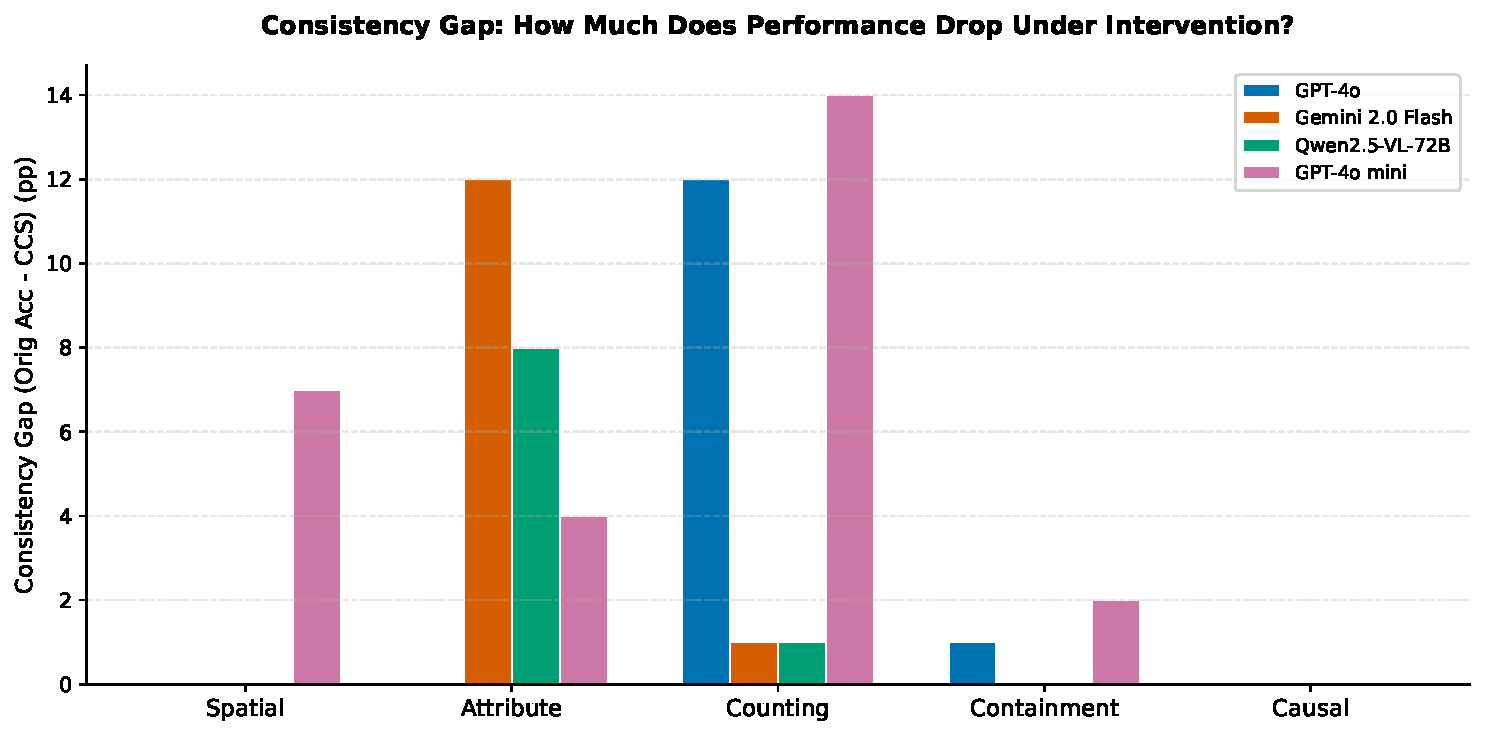
\includegraphics[width=\columnwidth]{../figures/consistency_gap.pdf}
\caption{\textbf{Consistency gap} (original accuracy $-$ \ccs) by category. Larger gaps indicate models that give correct answers to individual images but fail to maintain consistency across the paired intervention.}
\label{fig:gap}
\end{figure}

\Cref{fig:gap} shows the consistency gap per category. Key observations:
\begin{itemize}
\setlength\itemsep{0pt}
\item \textbf{Counting} has the largest gap for GPT-4o (12 pp) and GPT-4o mini (14 pp): these models often get the original count right but fail on the intervened count (or vice versa).
\item \textbf{Attribute binding} shows a notable gap for Gemini (12 pp), suggesting Gemini sometimes recognizes colors correctly but is confused when the same shape appears in a different color.
\item \textbf{Spatial and containment} have near-zero gaps across all models---when these models succeed on one image, they consistently succeed on both.
\end{itemize}

\subsection{Negative Control Analysis}

\begin{figure}[t]
\centering
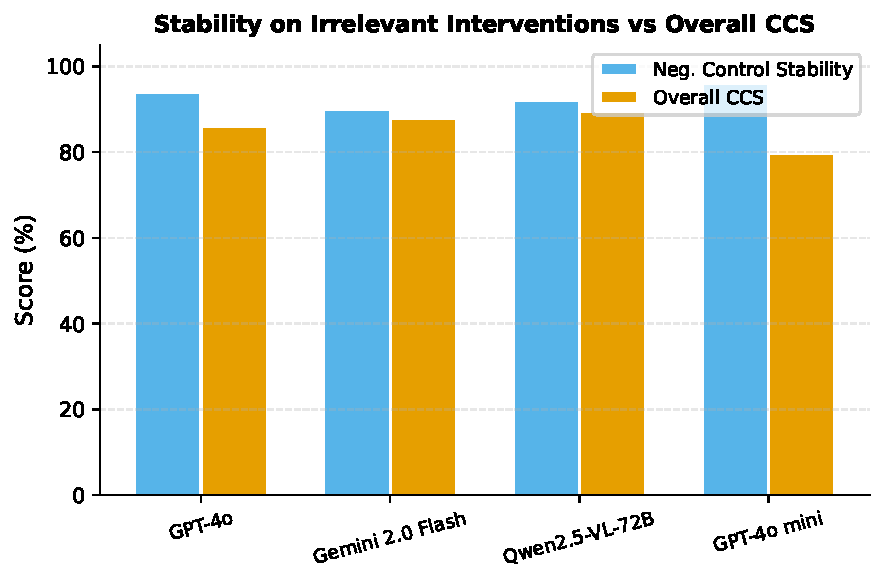
\includegraphics[width=\columnwidth]{../figures/negative_control.pdf}
\caption{\textbf{Negative control stability.} Models should maintain the same answer when irrelevant distractors are added. All models achieve 90--96\% stability, indicating they rarely hallucinate or flip answers due to irrelevant visual changes.}
\label{fig:negctrl}
\end{figure}

\Cref{fig:negctrl} shows that all models maintain high stability (90--96\%) on negative controls, where an unrelated shape is added far from the target. This confirms that the failures observed in \Cref{tab:category} are genuine reasoning failures, not artifacts of visual distraction sensitivity.

\subsection{Qualitative Error Analysis}

\begin{figure}[t]
\centering
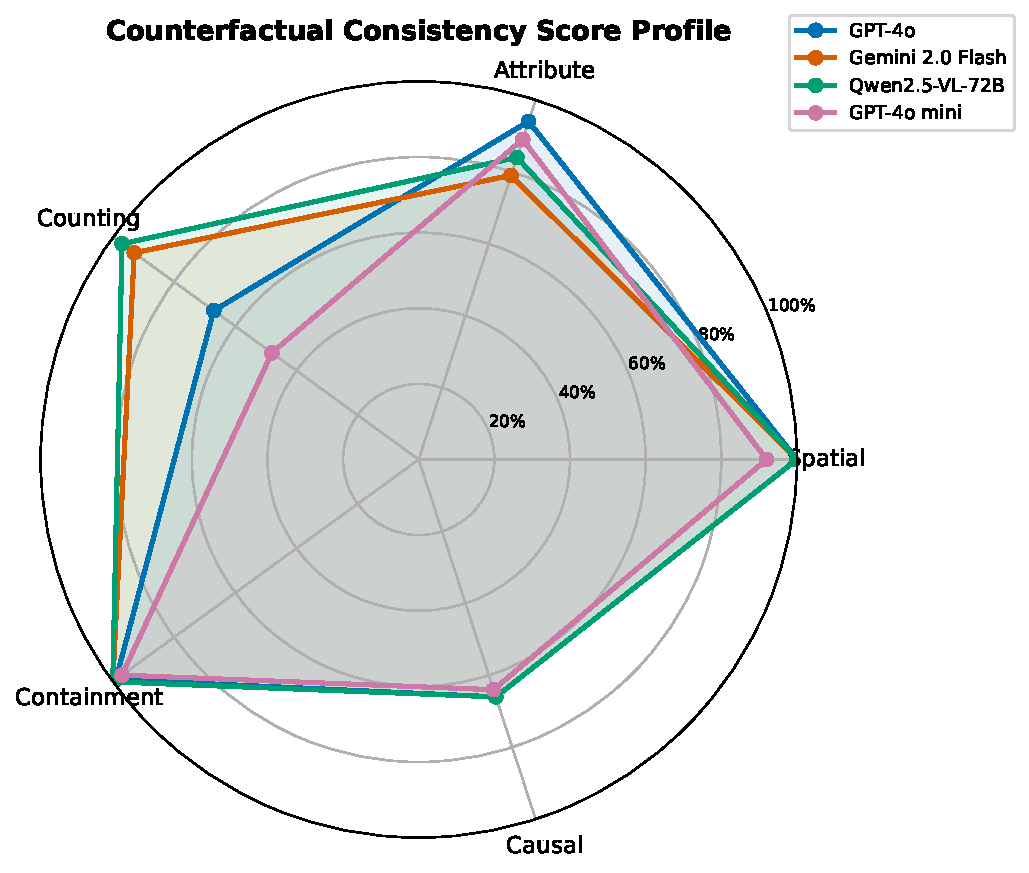
\includegraphics[width=\columnwidth]{../figures/radar_ccs.pdf}
\caption{\textbf{\ccs profile} across five task categories. The ``dent'' in the causal dimension is universal; other dimensions show model-specific strengths.}
\label{fig:radar}
\end{figure}

\Cref{fig:radar} visualizes the \ccs profile as a radar chart. All models exhibit a characteristic ``dent'' in the causal dimension. GPT-4o mini shows an additional dent in counting, while Gemini shows one in attribute binding. Qwen2.5-VL-72B has the most uniform profile, but still shares the causal weakness.

Manual inspection of causal-arrow errors reveals two failure patterns: (1)~\textbf{arrow blindness}: the model names a shape but ignores the arrow entirely, defaulting to the most salient or centered object; (2)~\textbf{sticky answers}: the model gives the same answer for both original and intervened images, suggesting it encodes the scene layout but not the arrow direction.

For counting errors, models often err by $\pm$1 in scenes with 4+ objects, consistent with known subitizing limits~\cite{fu2024blink} and the difficulty of precise enumeration in VLMs.

%----------------------------------------------------------------------
\section{Discussion}
\label{sec:discussion}

\paragraph{Why counterfactual consistency matters.}
Standard accuracy metrics credit models for getting single questions right, but do not test whether the model's understanding is coherent across related scenarios. A model that answers ``3 circles'' in the original and ``3 circles'' in the intervened image (where there are now 4) scores 50\% accuracy but 0\% \ccs---revealing that it pattern-matches rather than counts. Our \ccs metric penalizes such inconsistency, providing a stricter test of genuine visual reasoning.

\paragraph{The causal reasoning gap.}
The universal $\leq$66\% \ccs on causal tasks is our most striking finding. Arrow-following requires the model to: (1) detect the arrow, (2) trace its direction, (3) identify the target. This is precisely the kind of relational, directional reasoning that BLINK~\cite{fu2024blink} and VSR~\cite{liu2023vsr} found lacking. Our results show this deficit persists even in 2025-era models, suggesting it may be architectural rather than a matter of scale.

\paragraph{Cheap benchmarking as a methodology.}
\method demonstrates that significant scientific insights can be obtained from trivially simple stimuli. The entire benchmark---generation, inference, and analysis---costs $<$\$12 and requires no GPU. This makes counterfactual testing accessible to any researcher and suggests a methodology for rapid, targeted probing of VLM capabilities as new models emerge.

\paragraph{Implications for cognitive foundations.}
From a cognitive science perspective~\cite{spelke2007core}, our results suggest VLMs have acquired ``core knowledge'' of spatial relations and containment but lack robust causal and quantitative reasoning. This mirrors developmental trajectories where children master spatial before causal reasoning~\cite{gopnik2004causal}, though the analogy should not be taken too literally.

\paragraph{Limitations.}
(1) Our scenes are simple geometric shapes, not natural images. While this is by design (for full control), it means our findings may not directly transfer to natural scenes. (2) We test four models; broader evaluation across open-source VLMs would strengthen the findings. (3) The causal subtask (arrow-following) may conflate arrow detection with causal reasoning proper. (4) Answer normalization introduces potential parsing errors, though our conservative matching reduces false positives.

%----------------------------------------------------------------------
\section{Conclusion}
\label{sec:conclusion}

We introduced \method, a fully synthetic, zero-cost benchmark for evaluating counterfactual consistency in vision-language models. By generating 550 paired images with precise visual interventions across five cognitive dimensions, we measure whether VLMs maintain consistent reasoning when scenes are modified. Our evaluation of four state-of-the-art VLMs reveals a heterogeneous failure landscape: spatial and containment reasoning are near-perfect, counting and attribute binding are model-dependent, and causal reasoning is universally weak. The Counterfactual Consistency Score (\ccs) provides a complementary metric to standard accuracy that captures reasoning coherence, and the $\leq$66\% causal \ccs shared by all models points to a systematic architectural limitation. We release all code, images, and evaluation scripts, and argue that cheap, controllable testbeds are an underutilized tool for understanding the cognitive foundations of multimodal AI.

%----------------------------------------------------------------------
{
    \small
    \bibliographystyle{ieeenat_fullname}
    \bibliography{references}
}

\end{document}
